%File: anonymous-submission-latex-2026.tex
\documentclass[letterpaper]{article} % DO NOT CHANGE THIS
\usepackage[submission]{aaai2026}  % DO NOT CHANGE THIS
\usepackage{times}  % DO NOT CHANGE THIS
\usepackage{helvet}  % DO NOT CHANGE THIS
\usepackage{courier}  % DO NOT CHANGE THIS
\usepackage[hyphens]{url}  % DO NOT CHANGE THIS
\usepackage{graphicx} % DO NOT CHANGE THIS
\urlstyle{rm} % DO NOT CHANGE THIS
\def\UrlFont{\rm}  % DO NOT CHANGE THIS
\usepackage{natbib}  % DO NOT CHANGE THIS AND DO NOT ADD ANY OPTIONS TO IT
\usepackage{caption} % DO NOT CHANGE THIS AND DO NOT ADD ANY OPTIONS TO IT
\frenchspacing  % DO NOT CHANGE THIS
\setlength{\pdfpagewidth}{8.5in} % DO NOT CHANGE THIS
\setlength{\pdfpageheight}{11in} % DO NOT CHANGE THIS
%
% These are recommended to typeset algorithms but not required. See the subsubsection on algorithms. Remove them if you don't have algorithms in your paper.
\usepackage{algorithm}
\usepackage{algorithmic}

%
% These are are recommended to typeset listings but not required. See the subsubsection on listing. Remove this block if you don't have listings in your paper.
\usepackage{newfloat}
\usepackage{listings}
\DeclareCaptionStyle{ruled}{labelfont=normalfont,labelsep=colon,strut=off} % DO NOT CHANGE THIS
\lstset{%
	basicstyle={\footnotesize\ttfamily},% footnotesize acceptable for monospace
	numbers=left,numberstyle=\footnotesize,xleftmargin=2em,% show line numbers, remove this entire line if you don't want the numbers.
	aboveskip=0pt,belowskip=0pt,%
	showstringspaces=false,tabsize=2,breaklines=true}
\floatstyle{ruled}
\newfloat{listing}{tb}{lst}{}
\floatname{listing}{Listing}
%
% Keep the \pdfinfo as shown here. There's no need
% for you to add the /Title and /Author tags.
\pdfinfo{
/TemplateVersion (2026.1)
}

% DISALLOWED PACKAGES
% \usepackage{authblk} -- This package is specifically forbidden
% \usepackage{balance} -- This package is specifically forbidden
% \usepackage{color (if used in text)
% \usepackage{CJK} -- This package is specifically forbidden
% \usepackage{float} -- This package is specifically forbidden
% \usepackage{flushend} -- This package is specifically forbidden
% \usepackage{fontenc} -- This package is specifically forbidden
% \usepackage{fullpage} -- This package is specifically forbidden
% \usepackage{geometry} -- This package is specifically forbidden
% \usepackage{grffile} -- This package is specifically forbidden
% \usepackage{hyperref} -- This package is specifically forbidden
% \usepackage{navigator} -- This package is specifically forbidden
% (or any other package that embeds links such as navigator or hyperref)
% \indentfirst} -- This package is specifically forbidden
% \layout} -- This package is specifically forbidden
% \multicol} -- This package is specifically forbidden
% \nameref} -- This package is specifically forbidden
% \usepackage{savetrees} -- This package is specifically forbidden
% \usepackage{setspace} -- This package is specifically forbidden
% \usepackage{stfloats} -- This package is specifically forbidden
% \usepackage{tabu} -- This package is specifically forbidden
% \usepackage{titlesec} -- This package is specifically forbidden
% \usepackage{tocbibind} -- This package is specifically forbidden
% \usepackage{ulem} -- This package is specifically forbidden
% \usepackage{wrapfig} -- This package is specifically forbidden
% DISALLOWED COMMANDS
% \nocopyright -- Your paper will not be published if you use this command
% \addtolength -- This command may not be used
% \balance -- This command may not be used
% \baselinestretch -- Your paper will not be published if you use this command
% \clearpage -- No page breaks of any kind may be used for the final version of your paper
% \columnsep -- This command may not be used
% \newpage -- No page breaks of any kind may be used for the final version of your paper
% \pagebreak -- No page breaks of any kind may be used for the final version of your paperr
% \pagestyle -- This command may not be used
% \tiny -- This is not an acceptable font size.
% \vspace{- -- No negative value may be used in proximity of a caption, figure, table, section, subsection, subsubsection, or reference
% \vskip{- -- No negative value may be used to alter spacing above or below a caption, figure, table, section, subsection, subsubsection, or reference

\setcounter{secnumdepth}{0} %May be changed to 1 or 2 if section numbers are desired.

% The file aaai2026.sty is the style file for AAAI Press
% proceedings, working notes, and technical reports.
%

% Title

% Your title must be in mixed case, not sentence case.
% That means all verbs (including short verbs like be, is, using,and go),
% nouns, adverbs, adjectives should be capitalized, including both words in hyphenated terms, while
% articles, conjunctions, and prepositions are lower case unless they
% directly follow a colon or long dash
\title{Mapping the Middle Ground: How Creators Accept, Enhance, and Reconfigure AI-Generated Designs}

%%\title{The Anatomy of a Choice: Expertise, Trust, and Decision Patterns in Human-AI Co-Creation}
\author{
    %Authors
    % All authors must be in the same font size and format.
    Written by AAAI Press Staff\textsuperscript{\rm 1}\thanks{With help from the AAAI Publications Committee.}\\
    AAAI Style Contributions by Pater Patel Schneider,
    Sunil Issar,\\
    J. Scott Penberthy,
    George Ferguson,
    Hans Guesgen,
    Francisco Cruz\equalcontrib,
    Marc Pujol-Gonzalez\equalcontrib
}
\affiliations{
    %Afiliations
    \textsuperscript{\rm 1}Association for the Advancement of Artificial Intelligence\\
    % If you have multiple authors and multiple affiliations
    % use superscripts in text and roman font to identify them.
    % For example,

    % Sunil Issar\textsuperscript{\rm 2},
    % J. Scott Penberthy\textsuperscript{\rm 3},
    % George Ferguson\textsuperscript{\rm 4},
    % Hans Guesgen\textsuperscript{\rm 5}
    % Note that the comma should be placed after the superscript

    1101 Pennsylvania Ave, NW Suite 300\\
    Washington, DC 20004 USA\\
    % email address must be in roman text type, not monospace or sans serif
    proceedings-questions@aaai.org
%
% See more examples next
}

%Example, Single Author, ->> remove \iffalse,\fi and place them surrounding AAAI title to use it
\iffalse
\title{My Publication Title --- Single Author}
\author {
    Author Name
}
\affiliations{
    Affiliation\\
    Affiliation Line 2\\
    name@example.com
}
\fi

\iffalse
%Example, Multiple Authors, ->> remove \iffalse,\fi and place them surrounding AAAI title to use it
\title{My Publication Title --- Multiple Authors}
\author {
    % Authors
    First Author Name\textsuperscript{\rm 1},
    Second Author Name\textsuperscript{\rm 2},
    Third Author Name\textsuperscript{\rm 1}
}
\affiliations {
    % Affiliations
    \textsuperscript{\rm 1}Affiliation 1\\
    \textsuperscript{\rm 2}Affiliation 2\\
    firstAuthor@affiliation1.com, secondAuthor@affilation2.com, thirdAuthor@affiliation1.com
}
\fi


% REMOVE THIS: bibentry
% This is only needed to show inline citations in the guidelines document. You should not need it and can safely delete it.
\usepackage{bibentry}
% END REMOVE bibentry

\begin{document}

\maketitle

\begin{abstract}
Generative AI tools enable rapid visual concept generation but often encourage an oversimplified accept–reject mindset. This paper maps the “middle ground” of interaction by introducing and applying a six-decision framework—\textit{Accept, Enhance, Reconfigure, Integrate, Reject, Iterate}—that captures the nuanced ways humans engage with AI outputs. Through a quasi-experimental study with 60 participants (novices and experts) tackling conventional and unconventional prompts under varying time constraints, we analyze how expertise, prompt type, and cognitive modes influence iterative refinement. Our mixed-methods data reveals that \textit{Enhance} decisions dominate early stages, while experts favor major transformations (\textit{Reconfigure, Integrate}) to adapt novel AI outputs. While time constraints exert modest effects, trust and usefulness consistently rise over iterative cycles, underscoring how partial modifications deepen human–AI synergy. During “pain points” of low trust, System I thinkers tend to reject suggestions outright, whereas System II users often attempt reconfiguration first. By illuminating these fine-grained creative choices, our analysis informs the design of adaptive AI systems that guide novices, empower experts, and balance human authorship with algorithmic assistance. Ultimately, our findings demonstrate how a deeper understanding of co-creative dynamics can foster richer artistic engagement and more innovative design collaboration.
\end{abstract}

\section{Introduction}
Recent advances in Generative AI—exemplified by systems like Midjourney, DALL·E, and ChatGPT—have dramatically expanded opportunities for artistic and design-based collaboration between humans and machines~\cite{dwivedi2023opinion,giordano2024impact}. These tools enable rapid production of visual concepts, illustrations, and stylistic variations, potentially supporting human creativity in areas ranging from logo design and poster creation to concept art and brand ideation. Yet despite growing enthusiasm for these human–AI partnerships, research has often overlooked the micro-level decision points that shape how artistic output evolves in practice~\cite{creely2024creative,egon2023ai}. Specifically, much of the existing work relies on a simple accept/reject lens, which obscures more nuanced decisions—such as partially adopting AI outputs, reconfiguring them for style alignment, or discarding them outright when they conflict with an artist’s aesthetic vision~\cite{kim2023effect}.

To address this gap, we focus on the co-creative decision process: how and why humans choose to accept, reject, or modify AI-generated suggestions within creative workflows. Understanding these critical decision points~\cite{cao2022understanding} is vital because artistic endeavors often hinge on iterative exploration, creative flow, and evolving aesthetic goals. AI systems might propose visual elements that spark new ideas or frustrate creators if the outputs stray too far from their intent~\cite{saetra2024machine}. We argue that analyzing these fine-grained choices can illuminate not only the trust and usefulness that participants place in AI but also the underlying cognitive and affective processes driving creative collaboration. These can range from rapid, intuitive judgments (System I thinking) to more deliberate, analytical reasoning (System II thinking)~\cite{kahneman2011fast}, alongside affective responses like momentary frustration or delight.

While prior co-creative frameworks offer valuable insights into the macro-level design of human-AI collaboration, they often do not capture the micro-level, artifact-oriented decisions that shape creative work. For instance, prominent models like the Co-Creative Framework for Interaction design (COFI) provide a powerful lens for analysing system architecture, such as turn-taking and communication styles~\cite{rezwana2023designing}. However, such system-level frameworks are not intended to classify a user's specific choice to take an AI output and subtly alter its color palette (an action we term Enhance). To address this gap at the user-action level, we introduce a six-category taxonomy—\textit{Accept, Enhance, Reconfigure, Integrate, Reject, Iterate}—to capture the range of decisions humans make when working with generative AI. Table~\ref{tab:decision-categories} presents a concise overview. By highlighting incremental refinements, partial integrations, and major transformations, this taxonomy reflects the iterative nature of creativity~\cite{sawyer2006educating}. Importantly, we also consider time constraints, expertise, and prompt conventionality as key factors that influence these decision pathways. We operationalize prompt conventionality by distinguishing between Conventional tasks (e.g., a standard poster) and Unconventional tasks (e.g., a hybrid-style logo), which are pertinent variables for professionals working under real deadlines~\cite{hong2019artificial,tillmann2024artificial}. 
 
This research aims to answer four key questions:

\begin{itemize}
    \item RQ1: Which of the six co-creative decision categories (\textit{Accept, Enhance, Reconfigure, Integrate, Reject, Iterate}) are most frequently used, and how do they manifest throughout the iterative design process?
   \item RQ2: Under which conditions—time constraints, prompt type (Conventional vs. Unconventional), and user expertise (novice vs. expert)—do participants shift from minor modifications to major transformations or outright rejection?
    \item RQ3: How do trust and perceived usefulness evolve across iterative interactions, and how do they affect final creative outcomes?
    \item RQ4: How do `pain points' (moments of low trust or frustration) and different cognitive modes (System I vs. System II) shape critical decision points in co-creative tasks?
\end{itemize}

This study makes three principal contributions: first, we introduce and demonstrate the application of a fine-grained decision taxonomy for co-creative human–AI interactions, extending existing models by explicitly accounting for partial modifications, structural reconfigurations, and iterative refinements in artistic tasks. Second, we empirically demonstrate how expertise, prompt conventionality, and time pressure shape these decision patterns, providing evidence that domain knowledge and deliberation (System II) can facilitate deeper creative transformations (\textit{Reconfigure, Integrate}), whereas novices or those under time stress often resort to quick accept/reject choices (System I). Third, we also propose design implications for adaptive AI tools—including ethical considerations around authorship and ownership—suggesting how future creative platforms could mitigate “pain points” and better support human agency in the face of generative AI outputs. By aligning our experiments with a visual design context and tapping into both quantitative (interaction logs, trust/usefulness ratings) and qualitative (think-aloud protocols, interviews) data, our findings shed light on when and why humans choose to override or collaborate with AI in creative work.

\begin{table}[ht]
\centering
\caption{Decision categories used to classify user actions in the refinement phase}
\label{tab:decision-categories}
\begin{tabular}{lp{6cm}}
\hline
\textbf{Decision} & \textbf{Definition} \\
\hline
\textbf{\textit{Accept}} & Incorporate the AI-generated output with minimal or no changes. \\
\textbf{\textit{Enhance}} & Make small aesthetic or stylistic tweaks while retaining the core composition. \\
\textbf{\textit{Reconfigure}} & Overhaul or significantly alter the layout or concept, retaining partial elements. \\
\textbf{\textit{Integrate}} & Combine multiple AI-generated or user-created elements into a single cohesive artifact. \\
\textbf{\textit{Reject}} & Discard or completely abandon the AI output. \\
\textbf{\textit{Iterate}} & Request variations or upscales without altering the output's fundamental concept. \\
\hline
\end{tabular}
\end{table}

In the following sections, we first review the relevant literature on human–AI collaboration and co-creative decision-making (§2), then detail our quasi-experimental methodology (§3). Next, we present results (§4) followed by a discussion (§5) of broader theoretical and practical implications for creative AI and a conclusion (§6) outlining future research directions.

\section{Related Work}
Researchers have increasingly explored Generative AI in creative domains, highlighting how AI tools can both augment and occasionally constrain human artistic practice. While these studies acknowledge the transformative potential of AI suggestions—from style transfer in digital art to thematic ideation~\cite{dwivedi2023opinion,giordano2024impact}—many still concentrate on final outcomes rather than examining the granular processes through which humans iteratively accept, reject, or modify AI outputs~\cite{pena2021artificial,chen2019artificial}. This focus on final artifacts overlooks the rich spectrum of co-creative actions that unfold in artistic workflows, such as subtly enhancing, reconfiguring, or integrating AI-generated elements to align with an evolving creative vision~\cite{kim2023effect,takaffoli2024generative}.

Drawing on creative flow and co-creation frameworks, scholars emphasize that collaborative creativity often hinges on iterative feedback loops where human intuition meets algorithmic suggestions~\cite{sawyer2006educating,shaer2024ai}. The risk in this delicate process is that when practitioners are under pressure or uncertain, they may either over-rely on the system (accepting suboptimal outputs) or prematurely discard generative ideas (rejecting them outright). This can lead to missed opportunities for transformational creativity—the generation of ideas that fall outside the established conceptual space~\cite{boden2009creativity}. This risk may be heightened when users lack the “specific curiosity" to probe and reconfigure unexpected outputs, a key driver of creative breakthroughs~\cite{grace2015specific}. Capturing the precise decision points that foster such curiosity is therefore a central challenge. This has led to the development of specialized evaluation instruments, such as the Mixed-Initiative Creativity Support Index, designed to assess the quality of co-creative interaction beyond simple usability~\cite{lawton2023drawing}.

Within this interplay, the cognitive lens of System I vs. System II~\cite{kahneman2011fast} is highly relevant. Fast, intuitive thinking (System I) can accelerate an artist’s process but may lead to hasty acceptance of stylistically mismatched outputs~\cite{cao2022understanding}. Deliberative, analytical reasoning (System II) fosters the extensive reconfiguration needed for deeper synergy but demands additional time and confidence~\cite{haase2024human,zhou2024understanding}. This connects directly to expertise; experts are more likely to engage in System II thinking, exhibiting the curiosity needed to transform unexpected AI outputs rather than merely accepting or rejecting them. Studies further confirm that trust and perceived usefulness are critical factors shaping these decisions in visual design and beyond~\cite{dwivedi2023opinion}. The unconventional prompt scenario is particularly intriguing: when AI produces flawed or unexpected outputs, it can overwhelm novices but prompt experts to become more critical and creative in their reconfigurations~\cite{liu2021understanding,lai2023towards}.

Moreover, discussions on ethics, authorship, and ownership highlight that creatives increasingly question whose vision is ultimately represented in a co-created piece~\cite{xu2024artificial}. While some see AI as a collaborative muse, others worry about appropriation or losing personal style in the process. As AI-generated artifacts become more sophisticated, defining who should be credited—and how—remains a significant concern~\cite{formosa2024can}. This underscores the importance of detailed taxonomies for capturing not just final acceptance or rejection but also partial adoption or iterative refinement, since these choices directly relate to perceptions of creative agency.

These challenges have inspired valuable macro-level frameworks for understanding human-AI collaboration. For instance, the Co-Creative Framework for Interaction design (COFI) offers an invaluable lens for designing and analyzing the architecture of collaboration, modeling high-level aspects like turn-taking and communication styles~\cite{rezwana2023designing}. However, such system-level frameworks are not designed to classify the user's specific, artifact-oriented actions—the micro-decisions that form the building blocks of the creative process. For example, while COFI can describe a system’s interaction style, it would not classify a user’s choice to Enhance an AI-generated image by subtly changing its color palette, or to Reconfigure its composition while preserving a single element. Our work complements these essential high-level approaches by providing a user-centric, artifact-focused taxonomy that maps this “middle ground" of interaction. By focusing on the six distinct decisions in our framework, we aim to clarify when and why creators embrace or override AI-generated suggestions, providing new insights for both theoretical models of creative cognition and the practical design of adaptive AI interfaces.
\section{Methodology}
%======================================================================
% 3.1 Framework and Terminology
% This new subsection addresses reviewer feedback by defining key concepts 
% upfront and explaining the origin of the framework.
%======================================================================

\subsection{Framework and Terminology}
The six-decision framework was developed through a preliminary analysis of pilot studies and a review of literature on creative cognition and design actions. The initial categories were refined iteratively by two researchers who coded a sample of pilot interaction videos, merging and splitting categories until the final set of six decisions was established as being both comprehensive and mutually exclusive for the observed actions. The six decision categories that form the core of our framework—\textit{Accept, Enhance, Reconfigure, Integrate, Reject, Iterate}—are formally defined in Table~\ref{tab:decision-categories} in the Introduction. We also analyze decisions through the cognitive lens of System~I and System~II thinking~\cite{kahneman2011fast}. System~I refers to fast, intuitive, and heuristic-based judgments, while System~II involves slower, deliberate, and analytical reasoning. This is relevant for understanding if `pain points' in the creative process trigger immediate reactions or thoughtful problem-solving. Our method for classifying actions into these modes is detailed in Section~3.6.

\subsection{Research Design and Stimuli}

We employed a quasi-experimental design to investigate how participants choose to accept, reject, or modify AI-generated outputs. The study had two key experimental factors: time pressure (short vs. long) and prompt type (Typical (TYP) vs. Atypical (ATYP)). The time constraint was manipulated between subjects: 30 participants were allocated to a short time condition (30–60 seconds observation) and 30 to a long time condition (2–3 minutes observation). Prompt type was a within-subjects factor, with each participant addressing both a TYP and an ATYP prompt.

To operationalize our prompt types rigorously and move beyond subjective selection, we employed a two-stage validation process. First, a set of 200 candidate prompts was scored for semantic similarity against the LAION-5B dataset using CLIP embeddings~\cite{radford2021learning}. Prompts in the lowest quartile of similarity were flagged as potentially Atypical, while those in the highest quartile were flagged as potentially Typical. Second, a panel of five expert designers, who did not participate in the main study, rated the conceptual familiarity of all prompts on a 5-point scale. Only prompts where the quantitative (CLIP score) and qualitative (panel rating) measures agreed were selected for the final study. The order in which participants engaged with the TYP and ATYP prompts was counterbalanced across the sample to mitigate potential sequence effects.
\subsection{Participants}
We recruited 60 participants (mean age = 29.4, SD = 5.8; 32 female, 28 male) through two primary channels. First, we posted calls for participation on prominent online design forums, as well as social media groups devoted to visual design. Second, we circulated email invitations within university networks, specifically targeting departments in graphic design, digital art, and related creative disciplines. Individuals interested in participating completed a brief screening survey that assessed their professional design experience (in years) and familiarity with generative AI tools. Based on their self-reported experience, participants who had fewer than one year of professional design practice were labeled as novices (n = 30), whereas those reporting two or more years of experience were labeled as experts (n = 30). We did not exclude individuals who had prior exposure to Midjourney or similar AI platforms; however, we incorporated a standardized tutorial phase (detailed below) to ensure a consistent baseline of tool familiarity.
\begin{figure*}[htbp]
\centerline{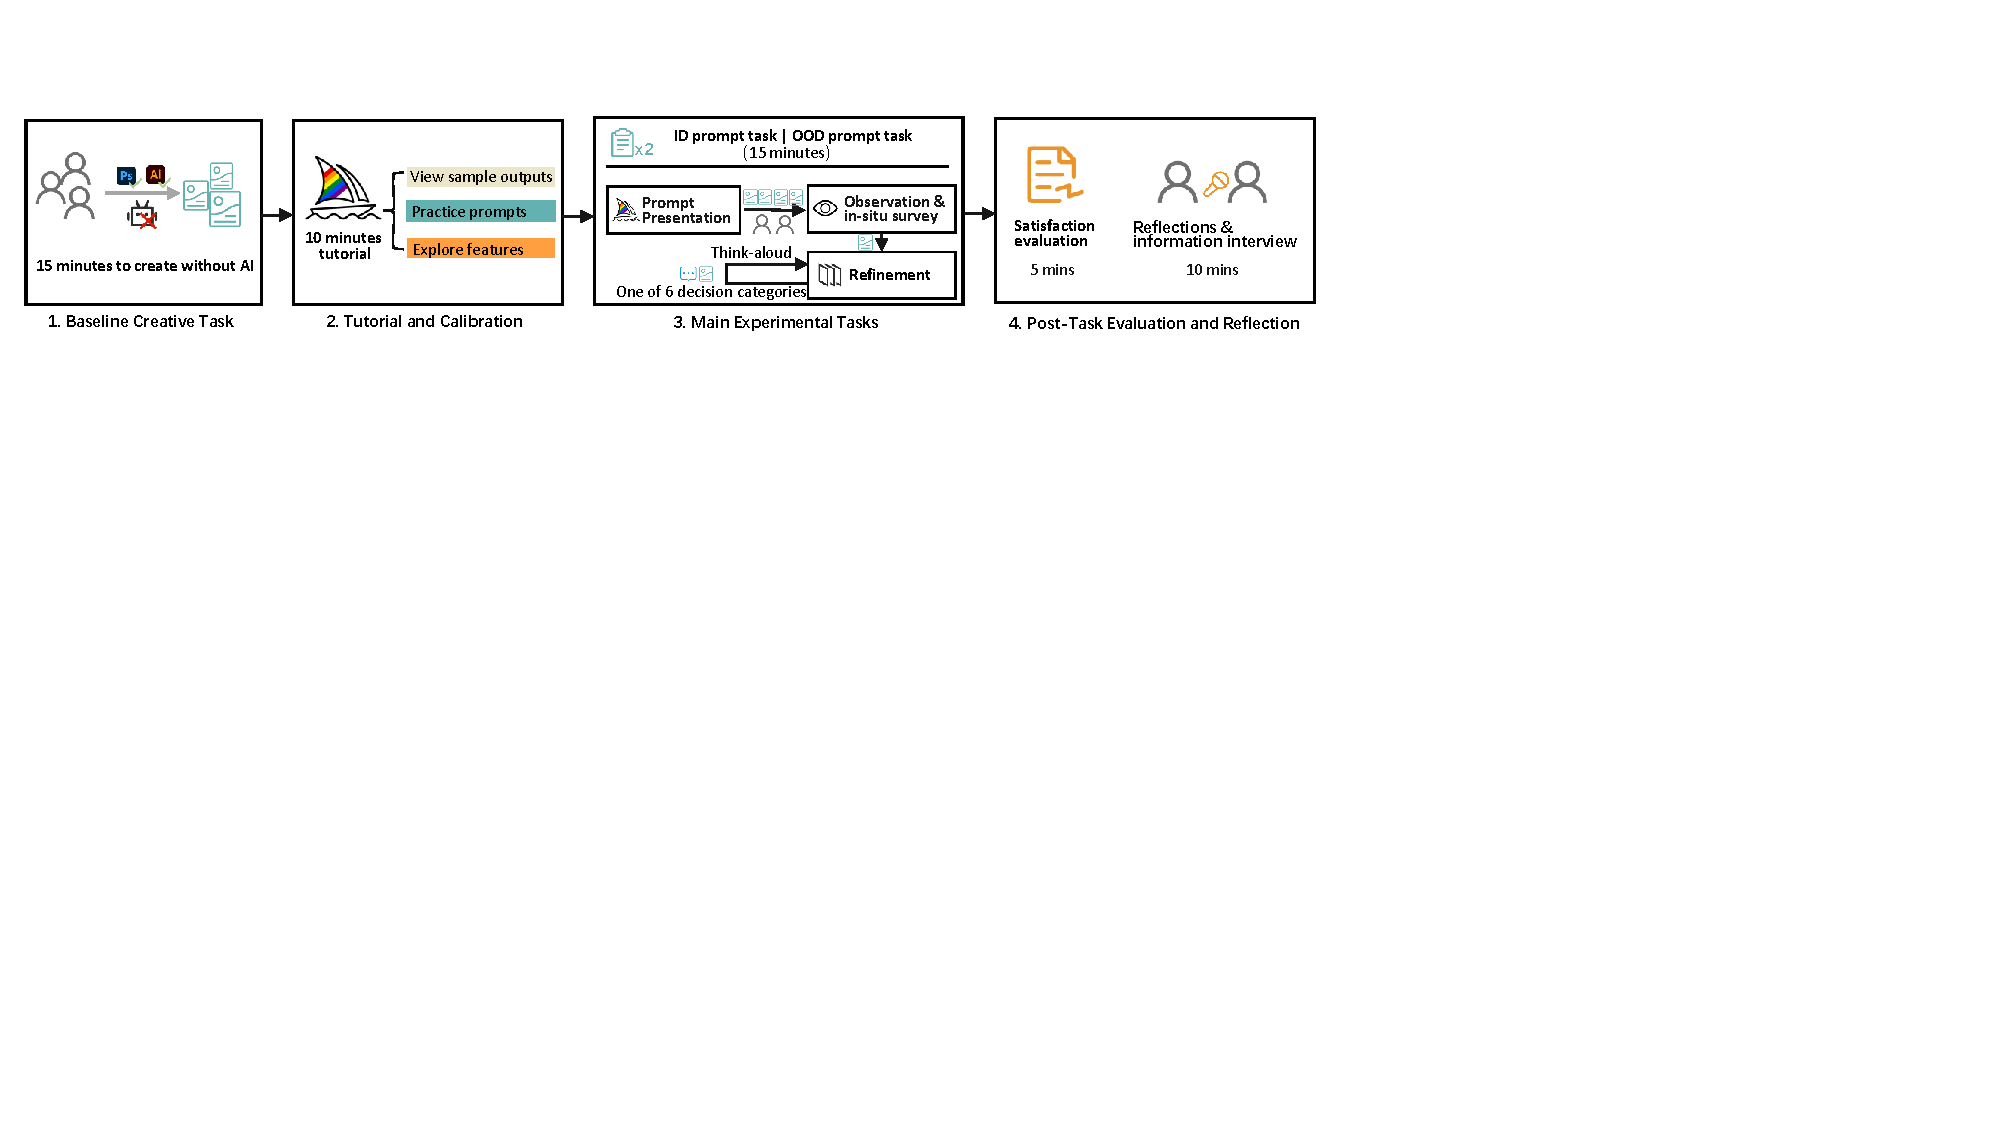
\includegraphics[width=1.0\textwidth]{framework.pdf}}
\caption{Detailed four-phase study design illustrating baseline creative tasks, a Midjourney tutorial and calibration, main experimental tasks under differing time constraints and prompt types, and post-task evaluation and reflection}
\label{researchframework}
\end{figure*}
%======================================================================
% 3.4 Procedure
% This section is revised to include justifications for tool choice and
% task timings, and critically, to correct the description of how 
% iterative trust/usefulness data was collected (addressing R3).
% A table mapping decisions to actions is also added (addressing R2).
%======================================================================

\subsection{Procedure}

Our study was organized into four main phases (see Figure~\ref{researchframework} for a schematic overview). We selected Midjourney as it is a state-of-the-art text-to-image model whose prompt-and-refine interaction style is representative of many contemporary generative AI tools. 
\subsubsection{Phase 1: Baseline Creative Task (Pre-Experiment)}
Participants completed a baseline design (a promotional poster) without AI. They had 15 minutes using any preferred digital design tool (Photoshop, Illustrator, etc.). This output served as a reference for each participant’s default style and capabilities in a no-AI scenario.

\subsubsection{Phase 2: Tutorial and Calibration}
Next, participants underwent a ten-minute Midjourney tutorial. They viewed sample outputs for both a Typical (e.g., “modern café poster”) and an Atypical (“abstract quantum mosaic”) prompt, practiced entering prompts, and explored variations/upscale features. This ensured all participants had basic proficiency with the tool.

\subsubsection{Phase 3: Main Experimental Tasks}
Each participant then undertook two creative tasks, each comprising Observation and Refinement sub-phases. One task involved a Typical prompt, whereas the other involved an Atypical prompt; the order was counterbalanced to control for learning or fatigue effects.

\paragraph{Prompt Presentation.} At the start of each task, participants viewed the assigned prompt. For instance, a Typical prompt might read “Design a modern café poster with a clean, minimal style,” whereas an Atypical prompt might state “Create a hybrid steampunk–minimalist logo for a futuristic bakery, combining intricate gears with simple geometric lines.” Participants typed the prompt into Midjourney to obtain four initial AI-generated outputs.

\paragraph{Observation Phase.} After the initial outputs appeared, participants were allocated a specific time to review them in accordance with their assigned condition. Those in the short time group had 30–60 seconds, whereas those in the long time group had 2–3 minutes. The observation windows were informed by usability research indicating that fast, impression-based inspection versus deliberate, analytical inspection differ by approximately a 4x time ratio. A visible countdown timer was provided to standardize this period.

\paragraph{Refinement Phase.} Following observation, participants entered an iterative refinement loop. To clarify the link between our abstract framework and concrete user actions, Table~\ref{tab:action-mapping} shows how each decision category was mapped to specific Midjourney commands or user behaviors. A critical part of this phase was capturing dynamic perceptions. After each major refinement decision (i.e., selecting one of the six categories from Table~\ref{tab:action-mapping}), participants were prompted to quickly re-rate their trust in the AI and the usefulness of its output on a 1-5 scale. This allowed us to track the evolution of these metrics throughout the creative process. Participants were asked to speak aloud during this phase, articulating their reasons for their choices. Both the screen activity and audio commentary were recorded. Participants continued iterating until they declared themselves satisfied or reached 15 minutes of total refinement time, whichever came first. After concluding the first prompt, they repeated the same procedure for the second prompt.


\begin{table}[htbp]
\centering
\caption{Mapping of decision categories to user actions.}
\label{tab:action-mapping}
\begin{tabular}{lp{6cm}}
\hline
\textbf{Decision} & \textbf{Corresponding Midjourney / User Action} \\
\hline
\textbf{\textit{Accept}} & Upscaling (U buttons) \& saving the image. \\
\textbf{\textit{Enhance}} & Making minor prompt edits (e.g., adding adjectives). \\
\textbf{\textit{Reconfigure}} & Major prompt rewrite or using remix mode. \\
\textbf{\textit{Integrate}} & Verbally noting the combination of ideas from multiple outputs. \\
\textbf{\textit{Reject}} & Using the re-roll button to discard the set. \\
\textbf{\textit{Iterate}} & Requesting variations (V buttons) of one image. \\
\hline
\end{tabular}
\end{table}
\subsubsection{Phase 4: Post-Task Evaluation and Reflection}
The final phase consisted of a brief (approximately 15-minute) evaluation and reflection. Participants completed a short survey assessing their satisfaction with each final design (Typical and Atypical), perceived creative synergy (on a 1–5 scale), and self-reported effort or cognitive load. This was followed by a semi-structured interview lasting about ten minutes, in which we asked participants to reflect on moments of frustration, low trust, or significant breakthroughs.\footnote{Questions included: “Which AI outputs felt most misaligned with your creative vision?” and “Was there a point where you considered abandoning the AI’s suggestions?”} We also collected optional demographic information such as educational background and design domain.

%======================================================================
% 3.5 Data Collection and Measures
% This section is revised to justify survey choices (TAM), acknowledge
% alternatives (MI-CSI), and list the specific emotion descriptors used,
% addressing feedback from Reviewers #1 and #2.
%======================================================================

\subsection{Data Collection and Measures}
Interaction logs automatically recorded each major decision (\textit{Accept, Enhance, Reconfigure, Integrate, Reject, Iterate}), along with timestamps and any textual prompts entered. Full-screen recordings at 1080p captured all on-screen actions, while synchronized audio recordings captured participants' think-aloud commentary. Trust and usefulness scales were adapted from the Technology Acceptance Model (TAM)~\cite{davis1989technology}. TAM was chosen for its robustness and to facilitate comparison with prior co-creation studies that use its core constructs~\cite{dwivedi2023opinion}. While newer instruments like the Mixed-Initiative Creativity Support Index (MI-CSI) exist~\cite{lawton2023drawing}, its 36 items were deemed too lengthy for our rapid, in-situ data capture during the iterative task. Affective responses were captured via a forced-choice selection from an 8-item list: \textit{intrigued, excited, amused, neutral, confused, annoyed, frustrated,} and \textit{bored}.

\subsection{Data Analysis}
Decision frequencies and transition patterns were compiled to chart typical co-creative paths. We then conducted mixed-effects logistic regressions to assess how time constraints (short vs. long), prompt type (Typical vs. Atypical), and expertise level (novice vs. expert) predicted decision outcomes. A repeated-measures ANOVA was employed to examine changes in trust and usefulness ratings over multiple refinement steps, while correlational analyses explored the link between these ratings and final design satisfaction.

To classify decisions as indicative of System I or System II thinking, we performed a post-hoc analysis of the behavioral data. Actions were coded as System I if they met two criteria: (1) they were executed in under 5 seconds from when the AI output was displayed, and (2) they were accompanied by fewer than 10 words of verbal reasoning in the think-aloud transcript. All other actions were coded as System II. Two researchers independently coded a subset of the data (20\% of sessions), achieving high inter-rater reliability for this classification (Cohen’s $\kappa$ = 0.80).

The think-aloud transcripts and post-task interview data were thematically coded following the six-phase protocol from Braun and Clarke~\cite{clarke2017thematic}. Two researchers independently coded the data, identified recurring patterns, and resolved disagreements through discussion to achieve high reliability (Cohen’s $\kappa$ = 0.84). This process identified three overarching themes explaining participants' strategies for resolving mismatches and responding to the AI: (1) Salvaging Potential, where users saw value in flawed outputs; (2) Confidence and Expertise, reflecting the user's self-assessed ability to "fix" the AI's work; and (3) Ownership Concerns, related to maintaining a personal artistic fingerprint.



\section{Results}
\subsection{Co-Creative Decision Patterns (RQ1)}
Our analysis revealed distinct preferences in how participants incorporated or dismissed AI-generated suggestions across multiple iterations. As demonstrated in Figure~\ref{fig:multipanel}(a), in the initial observation phase, 70\% of participants chose to engage with the AI output rather than accepting it outright. Correspondingly, initial trust and usefulness scores both averaged around 3.4 on a 5-point scale (Figure~\ref{fig:multipanel}(b)), indicating a cautiously optimistic attitude toward collaboration. Over subsequent iterations, \textit{Enhance} decisions dominated early design cycles, accounting for 51.67\ of all actions in the first iteration (p$<$.01). These enhancements gradually gave way to more decisive actions—particularly \textit{Accept}—after approximately five refinement rounds (Figure~\ref{fig:multipanel}(f)). By the eleventh iteration, 90\% of participants who continued iterating had converged on a final design, underscoring that persistent refinement typically led to a satisfactory co-created artifact.

A closer look at decision transitions using a Sankey diagram (Figure~\ref{fig:sankey}) revealed common multi-step pathways. For example, a frequent sequence observed in 10\% of all sessions was “\textit{Enhance → Iterate → Enhance → Iterate → Accept}.” This pattern was most prevalent among expert users working on Typical prompts, where \textit{Enhance} decisions alone constituted 31.36\% of all actions. Novice users, by contrast, exhibited a higher frequency of immediate acceptance (16.91\% for Typical prompts) or complete rejection (26.63\% for Atypical prompts), suggesting a more polarized approach to AI suggestions.

%======================================================================
% REVISED FIGURE 2 (Your 'Layout 20.pdf')
%======================================================================
\begin{figure}[htbp]
\centerline{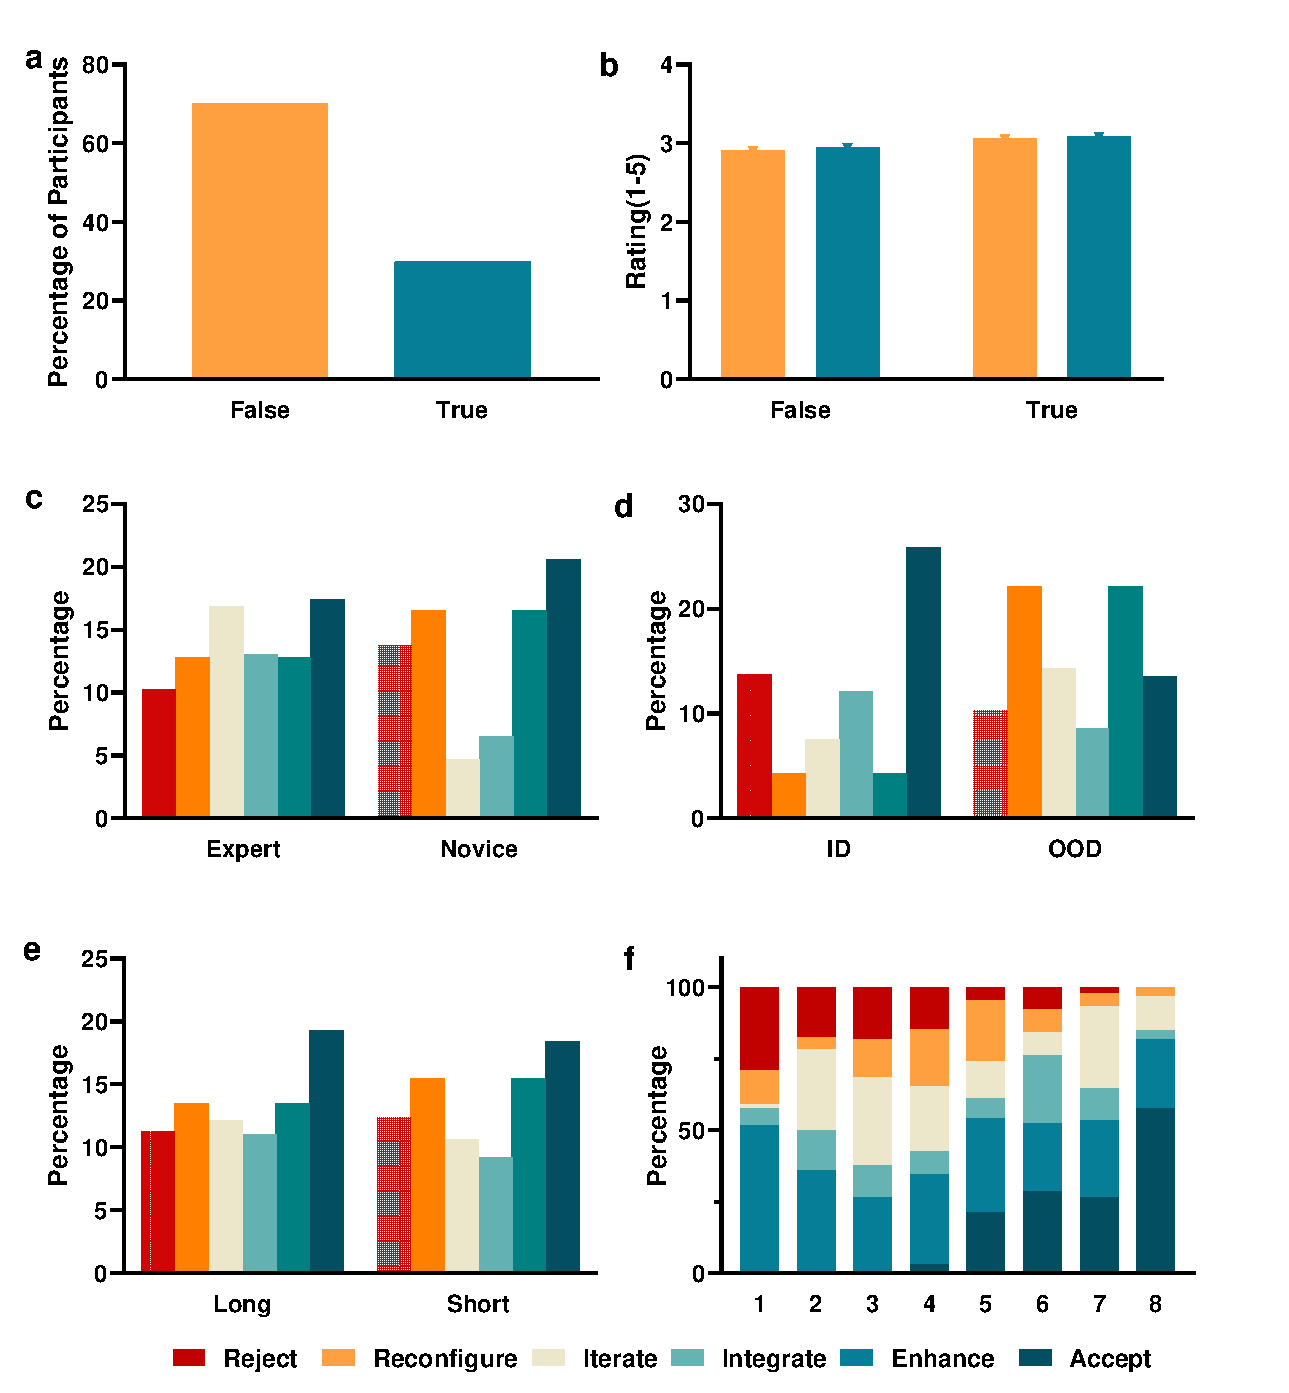
\includegraphics[width=0.53\textwidth]{Layout 20.pdf}} % I'm using the file name you provided.
\caption{\textbf{Overview of decision patterns and influencing factors.} \textbf{(a)}~Proportion of participants who immediately accepted the initial AI output (True) versus those who chose modification or rejection (False). \textbf{(b)}~Mean initial ratings for Trust and Usefulness (1-5 scale). \textbf{(c-e)}~Distribution of decision types by (c)~Expertise, (d)~Prompt Type, and (e)~Time Constraint. \textbf{(f)}~Evolution of decision types as a percentage of all actions across the first eight iterative steps.}
\label{fig:multipanel}
\end{figure}

%======================================================================
% REVISED FIGURE 3 (Your 'Sankey_output_3.pdf')
%======================================================================
\begin{figure}[htbp]
\centerline{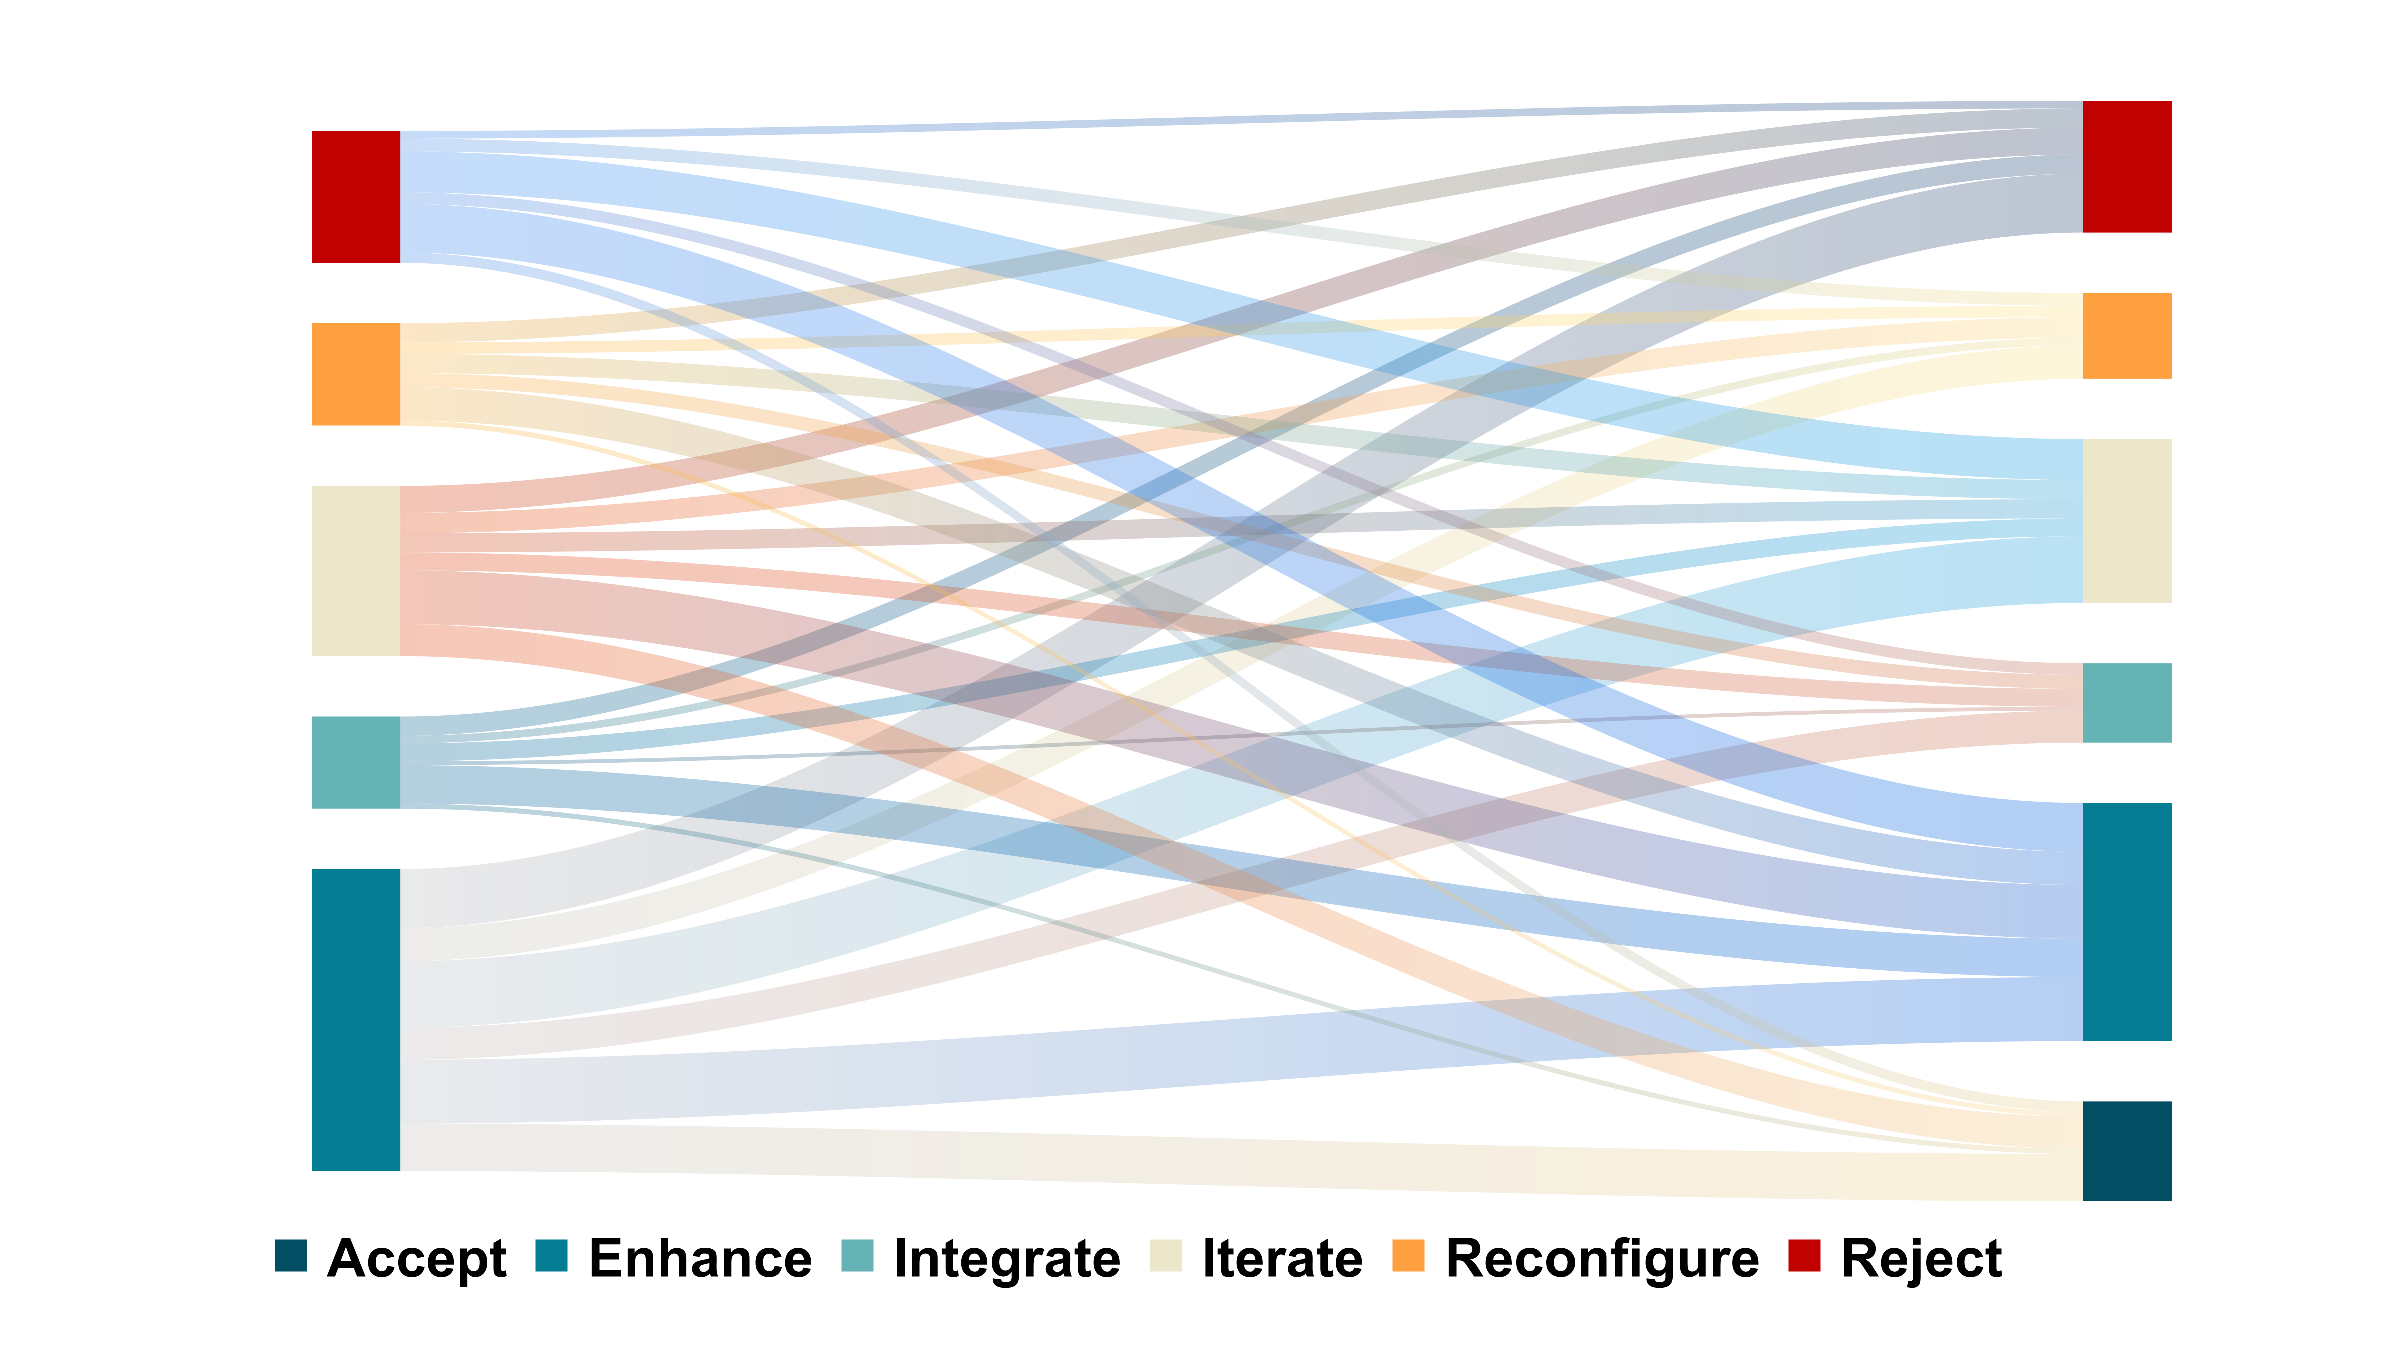
\includegraphics[width=0.48\textwidth]{Sankey_output_3.pdf}}
\caption{The flow of decisions between consecutive steps. The width of each flow is proportional to the frequency of that specific transition (e.g., from \textit{Enhance} to \textit{Iterate}).}
\label{fig:sankey}
\end{figure}

\subsection{Impact of Contextual Factors on Decision-Making (RQ2)}
Expertise and prompt type emerged as crucial influences on co-creative decisions, whereas time constraints had subtler effects. Chi-square analyses revealed that expert users performed major transformations (“\textit{Reconfigure}” or “\textit{Integrate}”) significantly more often than novices (29.92\% vs. 11.25\%, p$<$.001) (Figure~\ref{fig:multipanel}(c)). Experts also showed higher use of reconfiguration strategies for Atypical prompts (19.37\%) than for Typical prompts (13.61\%), whereas novices rarely attempted reconfiguration in Typical tasks (0\%). This disparity indicates that domain familiarity emboldened experts to experiment with AI outputs, even when those outputs were unconventional.

Prompt type similarly affected user behavior. Atypical prompts elicited a rejection rate of 22.17\%, compared to only 4.26\% for Typical prompts (p$<$.001) (Figure~\ref{fig:multipanel}(d)). Qualitative feedback suggested that novices, in particular, often dismissed Atypical outputs they perceived as too divergent from their initial vision. Nevertheless, some experts harnessed these “outlier” suggestions as opportunities for transformational creativity~\cite{boden2009creativity}. Thus, under Atypical prompts—especially for novices—there is a heightened likelihood of outright rejection.

Time constraints exerted only minor influences overall. While participants under long observation windows showed a marginally higher rate of major modifications (24.86\% vs. 21.27\% in the short condition), these differences did not reach statistical significance (all p$>$.05 ) (Figure~\ref{fig:multipanel}(e)). Still, interview data hinted that additional time gave certain participants space for deeper reflection, especially on Atypical tasks.

%======================================================================
% REVISED FIGURE 4 (Your 'Layout 21.pdf')
%======================================================================
\begin{figure}[htbp]
\centerline{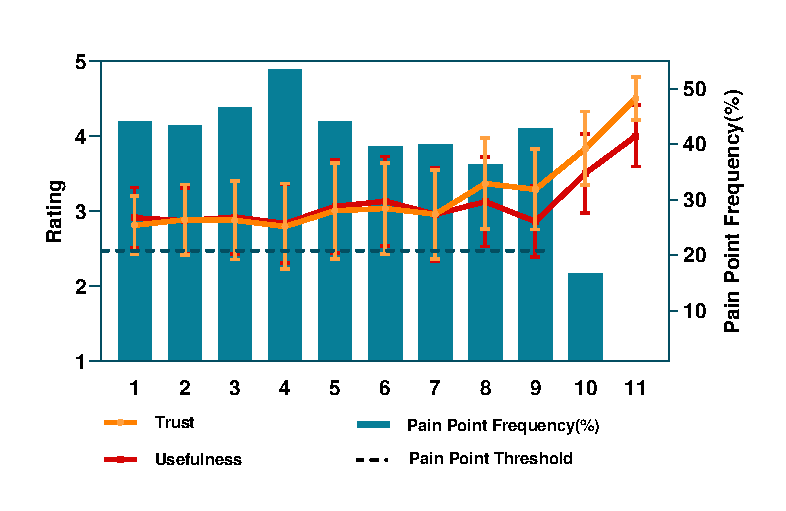
\includegraphics[width=0.53\textwidth]{Layout 21.pdf}} % I'm using the file name you provided.
\caption{\textbf{Evolution of Trust, Usefulness, and Pain Point Frequency across iterations.} Line plots show the mean ratings for Trust (orange) and Usefulness (red) on a 1-5 scale (left axis), with error bars representing standard error. The bar chart shows the percentage of sessions currently experiencing a "pain point" at each iteration (teal bars, right axis). A pain point is defined as an instance where a user's Trust and Usefulness ratings both fall below the 2.5 threshold (dotted line).}
\label{fig:trust_evolution}
\end{figure}

\subsection{Trust and Usefulness Dynamics (RQ3)}
Trust and usefulness ratings evolved in three discernible phases (Figure~\ref{fig:trust_evolution}). They dipped slightly below 3.0 during early iterations—likely reflecting initial skepticism—then stabilized in the 2.8–3.1 range through mid-phase experimentation, and ultimately climbed to around 4.0 by the final iterations (p$<$.001 for overall improvement). This upward trend suggests that iterative refinements can foster stronger user–AI synergy over time.

Decision-type analyses showed that \textit{Accept} mapped to the highest trust and usefulness means (4.00 and 3.76, respectively), while \textit{Reject} was associated with the lowest (2.13 and 2.27). Intriguingly, \textit{Reconfigure} carried relatively low trust (2.57) but moderate usefulness (2.75), implying that users might undertake major modifications when they doubt the AI’s style alignment but still see potential value in its output. This finding highlights that participants may heavily alter AI suggestions rather than discarding them outright, so long as they perceive some underlying utility.

\subsection{Pain Points and Cognitive Processing Patterns (RQ4)}
Nearly 44.3\% of all creative sessions contained “pain points,” as defined by moments when trust and usefulness dropped below 2.5 (Figure~\ref{fig:trust_evolution}). Participants responded differently depending on their cognitive style. Those leaning on System I thinking tended to reject AI outputs outright (24.76\% of low-trust decisions), whereas those engaging System II thinking more frequently opted for reconfiguration (14.29\%) or integration (7.94\%). A repeated-measures analysis indicated that System II thinkers also recovered higher trust and usefulness scores—on average—within 4.39 iterations following a pain point. When novices used System I thinking, they rejected AI outputs 24.76\% of the time; in contrast, System II thinkers pivoted to reconfiguration (14.29\\%). Frustration episodes often lead to immediate rejections unless the user adopts a more deliberative mode of thinking.

The results show that co-creative decisions with AI are neither binary nor static. Instead, they evolve through iterative feedback loops shaped by expertise, prompt type, and the gradual build-up of trust and usefulness. The interplay between System I/II thinking further enriches this dynamic, revealing how some users embrace a rapid trial-and-error process, while others prefer deliberate modifications to salvage challenging AI outputs.

%%%  这个部分可以详细扩展
\subsection{Insights from Interviews}
To complement our quantitative findings, we conducted semi-structured interviews (approximately 15 minutes each) aimed at capturing participants’ subjective experiences—particularly their motivations for adopting, rejecting, or transforming AI outputs. Three main themes emerged:

\paragraph{Salvaging Potential:} A recurring idea, especially among expert participants, was the notion of “salvaging” AI outputs that seemed initially misaligned. For example, one expert (P26) stated, “It only needed a slight nudge to get the color scheme right. I didn’t want to discard the design entirely because it had promise.” This readiness to persist with unconventional suggestions helps explain why experts frequently opted for major transformations (\textit{Reconfigure} or \textit{Integrate}) rather than discarding seemingly off-track outputs. They described a willingness to invest additional time and effort once they perceived something “interesting” (P19) in an AI-generated concept.

\paragraph{Confidence and Expertise:} Novice users, on the other hand, highlighted a sense of uncertainty when outputs felt too different from their envisioned style. One novice participant (P11) remarked, “I’m not sure how to fix it once it goes off-track. It’s easier to just reject it and start over.” Statements like these echo the higher rejection rates we observed in unconventional tasks. While expert participants often treated unconventional outputs as creative opportunities, novices were more likely to interpret them as lost causes, citing limited knowledge about how to reconcile aesthetic misalignments.

\paragraph{Ownership Concerns:} Finally, both experts and novices expressed concerns about creative ownership. For instance, one novice (P38) worried that “too much AI influence” would lead to a design that no longer felt personal, emphasizing a desire to preserve “my own artistic fingerprint.” This concern often underpinned participants’ inclination to \textit{Enhance} or \textit{Iterate} rather than \textit{Accept}. Some participants also noted that integrating AI outputs had practical advantages (e.g., speed, technical polish) but risked diluting their sense of authorship. Ultimately, participants sought a careful balance between leveraging the AI’s strengths and maintaining individual creative control.

\section{Discussion}

Our findings shed light on the nuanced and multifaceted ways in which humans navigate co-creative processes with generative AI in a visual design context. By moving beyond a simplistic accept–reject model, this study charts the complex decision pathways that unfold during artistic workflows. The application of our six-decision framework reveals not only what choices creators make but also begins to explain why they make them, pointing to the interconnected roles of domain expertise, iterative trust-building, and the deeply personal nature of creative ownership.

\paragraph{Expanding the Co-Creative Decision Lens.}
The primary contribution of this work is the introduction and application of a granular six-category taxonomy that captures the reality of creative engagement. In contrast to a binary outcome, our findings show that the co-creative process is a dynamic journey filled with micro-decisions. This aligns with Sawyer’s (2006) concept of "collaborative emergence," which posits that creativity flourishes through repeated, small-scale cycles of idea generation, critique, and refinement. We observed this directly: participants rarely accepted initial outputs outright. Instead, they moved toward deeper engagement with the AI after first testing incremental tweaks (\textit{Enhance}) or requesting subtle variations (\textit{Iterate}). These seemingly minor actions served to build momentum, gradually honing an artifact that felt more personally meaningful and aligned with their evolving vision. This underscores that the "middle ground" between acceptance and rejection is not empty, but rather a rich space of productive creative labor.

\paragraph{The Role of Expertise in Navigating Creative Uncertainty.}
Our results strongly highlight how domain expertise shapes a creator's strategy for dealing with the uncertainty inherent in generative AI. The most significant behavioral divergence was that expert designers were far more willing to pursue major transformations (\textit{Reconfigure} or \textit{Integrate}), especially when confronted with Atypical prompts that might initially appear misaligned or flawed. This finding resonates deeply with foundational research in design cognition. As Cross (2004) has argued, a key differentiator of design expertise is the ability to frame and structure ill-defined problems. Our experts demonstrated this by treating strange AI outputs not as errors, but as ill-defined starting points. Furthermore, their readiness to "salvage" partial ideas mirrors the findings of Suwa et al. (2000), who observed that expert designers are adept at leveraging "unexpected discoveries" as a vehicle to reframe design requirements and spark new ideas.

In contrast, novices more frequently dismissed off-track outputs, suggesting they experienced a faster "drop-off" in trust when Atypical suggestions veered too far from their comfort zone. This divergence reflects the two cognitive modes: novices often defaulted to rapid, heuristic judgments (System I) that yielded quick rejections, likely due to a higher cognitive load and a lack of established schemas for fixing novel problems. Expert participants, backed by their extensive domain knowledge, appeared more capable of engaging in reflective, deliberative reconfiguration (System II), confidently transforming the AI's unexpectedness into a creative opportunity.

\paragraph{Building and Repairing Trust Through Iteration.}
The dynamic evolution of trust and perceived usefulness provides another key insight. Our findings show these metrics are not static; they improved significantly with iterative engagement, underscoring that sustained interaction can recalibrate a user's perception of an AI partner~\cite{buccinca2024optimizing,bansal2023workshop}. The process often began with skepticism, but repeated enhancements and integrations—even minor ones—fostered a sense of collaborative momentum and growing confidence in the AI's potential. However, our study also identified a critical "trust tipping point." This reflects a continuous, often subconscious, process of "trust calibration"~\cite{cao2022understanding}, where participants weigh the potential time cost of a major reconfiguration against the anticipated creative benefit. When they deemed further edits unlikely to bridge the gap between the AI’s output and their internal vision, outright rejection became the more cognitively efficient path.

\paragraph{Balancing Creative Ownership and Machine Assistance.}
The qualitative data from our interviews revealed pervasive concerns about balancing AI-derived efficiency with the preservation of personal authorship—a tension central to recent research on AI-facilitated creativity~\cite{xu2024artificial,formosa2024can}. Participants from both novice and expert groups expressed wariness of ceding too much control, articulating a desire to maintain their "own artistic fingerprint." In practice, this apprehension manifested as a deliberate preference for partial modifications, even when a near-finished design could have been accepted "as is." This behavior suggests that the act of modifying an AI's output is not just about improving the artifact, but also about asserting creative agency and claiming a stake in the final product. It reinforces prior findings that humans value interpretive agency and expressive input in co-creative contexts~\cite{chen2019artificial,liu2021understanding}.

\paragraph{Design Implications.}
From a tool-design perspective, our findings emphasize the need for flexible, adaptive AI interfaces that cater to varying levels of expertise and shifting user trust. For novices encountering "pain points," systems might offer "guided reconfiguration" features, such as contextual tips, one-click stylistic adjustments, or component-swapping suggestions to help bridge the gap when an output appears off-track. For experts, platforms should provide more advanced customization controls that encourage bold transformations without forcing them to abandon an otherwise promising idea. This could include sophisticated prompting interfaces, version control systems for creative "forks," or tools for seamlessly blending elements from multiple AI generations.

\paragraph{Limitations and Future Directions.}
While this study provides key insights, its limitations must be acknowledged. Our sample, though balanced between novices and experts, was constrained in size, and our findings are situated within the specific domain of visual design. A significant limitation is our reliance on Midjourney, a proprietary, closed-source model. Our findings are therefore specific to its particular architectural biases and prompt-based interaction paradigm. Future work should explore whether these decision patterns hold with open-source models (e.g., Stable Diffusion) or with different interaction modalities like in-painting and direct canvas manipulation. Furthermore, the legal and ethical constraints of Midjourney’s terms of service regarding data usage and commercial rights may have implicitly influenced participants' attitudes towards ownership.

Future research should conduct larger-scale or longitudinal studies to track how novices’ comfort with reconfiguring unfamiliar outputs shifts over time with repeated AI exposure. Additional inquiries could explore whether our six decision types generalize to other creative domains, such as music composition or creative writing, and whether certain fields necessitate unique forms of partial adoption. Finally, examining algorithmic approaches to generate more "salvageable" Atypical outputs could be a fruitful direction for designing AI systems that better anticipate users’ aesthetic goals, thus reducing abrupt rejections and fostering a deeper, more resilient co-creative synergy.
\section{Conclusion}
Overall, this work underscores the multifaceted nature of human–AI co-creation. While generative AI tools can bolster creativity, their true impact hinges on thoughtful system design that accommodates user expertise, style preferences, and an evolving sense of ownership. The interviews, in particular, underscore that even a seemingly simple shift from \textit{Reject} to \textit{Enhance} may represent a user’s intent to safeguard creative agency. By offering partial reconfiguration tools, guiding novices through uncertain territory, and empowering experts to adapt unconventional outputs, future AI platforms could enable more transformative and personally meaningful outcomes. Ultimately, our findings reveal co-creative processes that are neither fully machine-driven nor purely human-led, but rather dynamic collaborations capable of yielding innovative, surprising, and artistically rich results.

\section*{Ethical Statement}
 All study procedures were approved by the corresponding institution’s Ethics Review Board. Participants were  informed that they could withdraw at any time without penalty. Interview transcripts were de-identified before analysis, and only aggregated findings were reported.

\bibliographystyle{aaai2026}
\bibliography{aaai2026}

\end{document}
